\subsection{Photovoltaic generator model} \label{sec:pv_gen_mod}
In general, two different PV generators are examined. Namely the AE Solar AE195SMM6-36 and the DAS Energy DAS145PF. Only one (primary) PV generator is used to suppliy the repeater radio infrastructure with electrical energy, with the second one serving as a backup. The backup PV generator is installed when the primary one fails to convert the required amount of electrical energy. This is the case, for example, if it gets damaged during an ongoing mission. Since both PV generators have a similar power output $P_\mathrm{PV}$, it is up to the OeWF to decide which one is used as the primary and which one as the backup. Excerpts from their data sheets can be found in the tables \ref{tab:table_ae_solar_pvg_specs} and \ref{tab:table_das_energy_pvg_specs}.
\begin{table}[h!]
	\centering
	\footnotesize
\begin{tabular}{|l|c|}
	\hline
	\multicolumn{2}{|c|}{\textbf{AE Solar AE195SMM6-36 specifications}} \\
	\hline
	PV cell type & 5BB Monocrystalline \\
	PV cell area & $156,75 \cdot 156,75\mathrm{mm}^2$ \\
	Number of PV cells & $36$ $(4 \cdot 9)$ \\
	Wind load & $244\mathrm{kg}\mathrm{m}^{-2}$ \\
	Mechanical load & $550\mathrm{kg}/\mathrm{m}^2$ \\
	Operating temperature & $-40^\circ \mathrm{C}$ to $85^\circ \mathrm{C}$ \\
	\hline
 	Maximum system voltage & $1000\mathrm{V}$ \\
	Maximum series fuse rating & $10\mathrm{A}$ \\
	Short-circuit current & $9,79\mathrm{A}$ \\
	Open-circuit voltage & $25,87\mathrm{V}$ \\
	MPP current & $9,11\mathrm{A}$ \\
	MPP voltage & $21,41\mathrm{V}$ \\
	Nominal MPP power & $195,0\mathrm{W}$ (peak) \\
	NOCT & $45\pm2 ^\circ \mathrm{C}$ \\
	Efficiency & $19,25\%$ \\
	\hline
	Temperature coeff. for $P_{\mathrm{MPP}}$ & $-0,380 \%^\circ \mathrm{C}^{-1}$ \\
	Temperature coeff. for $U_{\mathrm{OC}}$ & $-0,290 \%^\circ \mathrm{C}^{-1}$ \\
	Temperature coeff. for $I_{\mathrm{SC}}$ & $0,050 \%^\circ \mathrm{C}^{-1}$ \\
	\hline
\end{tabular}
	\caption{Excerpt from the data sheet of the AE Solar AE195SMM6-36 PV generator at STC \cite{ae_solar:2019}.}
	\label{tab:table_ae_solar_pvg_specs}
\end{table}
\begin{table}[h!]
	\centering
	\begin{tabular}{|l|c|}
	\hline
	\multicolumn{2}{|c|}{\textbf{DAS Energy DAS145PF photovoltaic generator}} \\
	\hline
 	Solar cells & 3BB polycrystalline solar cells\\
	Number of solar cells & $36$ $(4 \times 9)$ \\
	Module length & $1549\mathrm{mm}$ \\
	Module width & $673\mathrm{mm}$\\
	Operating temperature range & \numrange{-40}{85}$^\circ \mathrm{C}$ \\
	Cables & $2 \times 4\mathrm{mm}^2, 900\mathrm{mm}$ \\
	\hline
	Maximum system voltage & 1000V \\
	Maximum over current protection & 20A \\
	$I_{\mathrm{SC}}$ & 8,56A \\
	$I_{\mathrm{MPP}}$ & 8,09A \\
	$U_{\mathrm{OC}}$ & 22,76V \\
	$U_{\mathrm{MPP}}$ & 18,15V \\
	\hline
	Temperature coefficient $P_{\mathrm{MPP}}$ & $-0,383 \mathrm{\% / ^\circ C}$ \\
	Temperature coefficient $U_{\mathrm{OC}}$ & $-0,310 \mathrm{\% / ^\circ C}$ \\
	Temperature coefficient $I_{\mathrm{SC}}$ & $0,051 \mathrm{\% / ^\circ C}$ \\
	\hline
\end{tabular}
	\caption{Excerpt from the data sheet of the DAS Energy DAS145PF PV generator at STC \cite{das_energy_2017}.}
	\label{tab:table_das_energy_pvg_specs}
\end{table}

As can be seen from the results of the \MAPLE source code in the appendix \ref{sec:maple_code}, it makes little difference for the first few decimal places if the model is approximated with the Jacobian matrix. In the \MAPLE source code, the caluclations are performed for the AE Solar AE195SMM6-36 PV generator, with its PV cell temperature being $\vartheta_\mathrm{C} = 25^\circ\mathrm{C}$ and the total irradiance onto its inclined surface being $E_\mathrm{G} = 200\mathrm{Wm}^{-2}$. These results can be replicated for the DAS Energy DAS145PF PV generator and for other values of $\vartheta_\mathrm{C}$ and $E_\mathrm{G}$ as well. Therefore, it can be said that the starting values shown in the equation (\ref{eq:U_OC_I_S_zero}) suffice as a good approximation for the PV generator's open-circuit voltage $U_\mathrm{OC}$ and reverse saturation current $I_\mathrm{S}$. This is because $I_\mathrm{S}$ is usually very small \cite{Mertens:2015, Wagner:2018}. 

The results for the modeled current-voltage and power-voltage characteristics of the AE Solar AE195SMM6-36 PV generator, depending on either the total irradiance onto its inclined surface $E_\mathrm{G}$ or on its PV cell temperature $\vartheta_\mathrm{C}$, can be seen in the figures \ref{fig:image_curr_volt_irr_ae_solar}, \ref{fig:image_power_volt_irr_ae_solar}, \ref{fig:image_curr_volt_temp_ae_solar} and \ref{fig:image_power_volt_temp_ae_solar}. If it depends on $E_\mathrm{G}$ it is assumed that $\vartheta_\mathrm{C} = 25^\circ\mathrm{C}$ is constant, and if it depends on $\vartheta_\mathrm{C}$ it is assumed that $E_\mathrm{G} = 1000\mathrm{Wm}^{-2}$ is constant. These constant vlaues for $\vartheta_\mathrm{C}$ and $E_\mathrm{G}$ were chosen because they represent the STCs. Identically, the results for the DAS Energy DAS145PF PV generator can be taken from the figures \ref{fig:image_curr_volt_irr_das_energy}, \ref{fig:image_power_volt_irr_das_energy}, \ref{fig:image_curr_volt_temp_das_energy} and \ref{fig:image_power_volt_temp_das_energy}. All results were obtained by programming the discussed model of a PV generator in \MATLAB.

From the current-voltage characteristics for different irradiance levels $E_\mathrm{G}$ of both PV generators shown in the figures \ref{fig:image_curr_volt_irr_ae_solar} and \ref{fig:image_curr_volt_irr_das_energy}, it can be seen that the short-circuit current $I_\mathrm{SC}$ decreases faster than the open-circuit voltage $U_\mathrm{OC}$. This is due to the fact that $I_\mathrm{Ph} = I_\mathrm{SC}$ is proportional to $E_\mathrm{G}$ (compare to equation (\ref{eq:i_ph_theta_phi})), while $U_\mathrm{OC}$ changes with the natural logarithm to it (compare to equations (\ref{eq:U_OC_theta_phi}) and \ref{eq:U_OC_I_S_zero})) \cite{Mertens:2015}.
\begin{figure}[h!]
	\centering
  	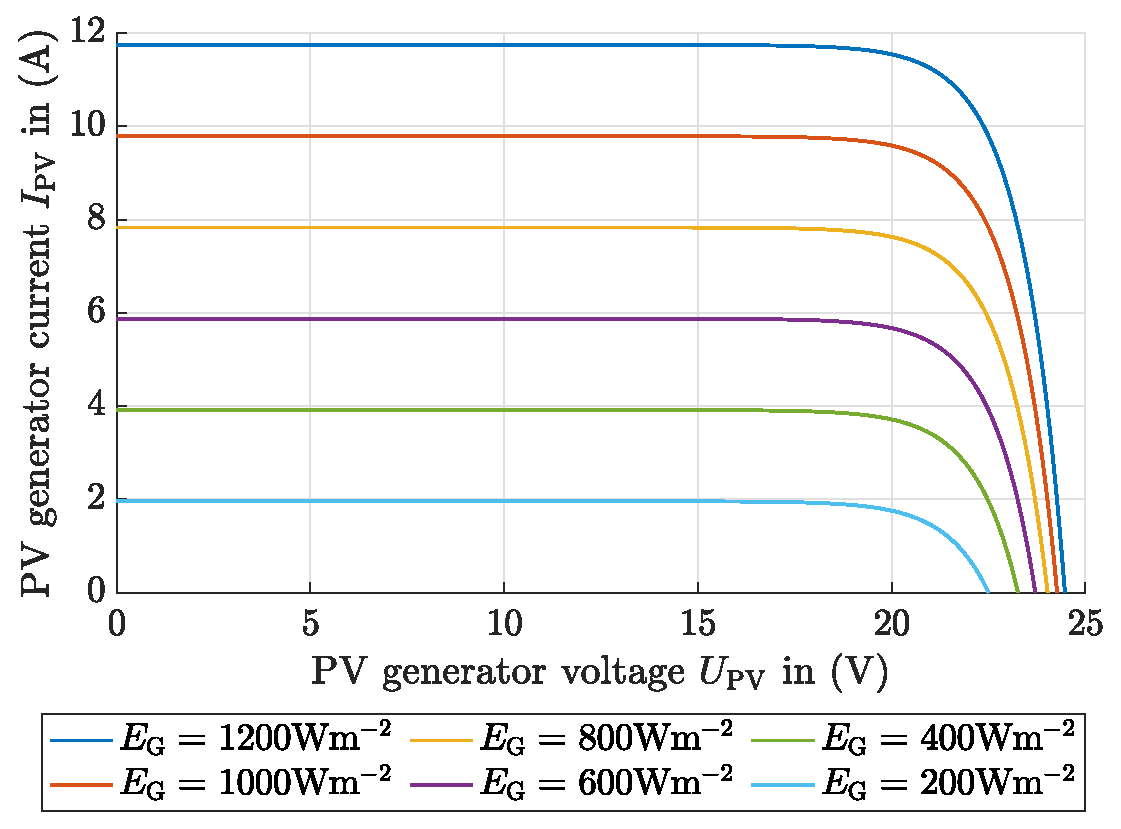
\includegraphics[width = 0.67\textwidth]{image_curr_volt_irr_ae_solar.eps}
  	\caption{Modeled current-voltage characteristic of the AE Solar AE195SMM6-36 PV generator, depending on the total irradiance onto its inclined surface $E_\mathrm{G}$. The PV cell temperature $\vartheta_\mathrm{C} = 25^\circ\mathrm{C}$ is assumed to be constant.}
	\label{fig:image_curr_volt_irr_ae_solar}
\end{figure}
\begin{figure}[h!]
	\centering
  	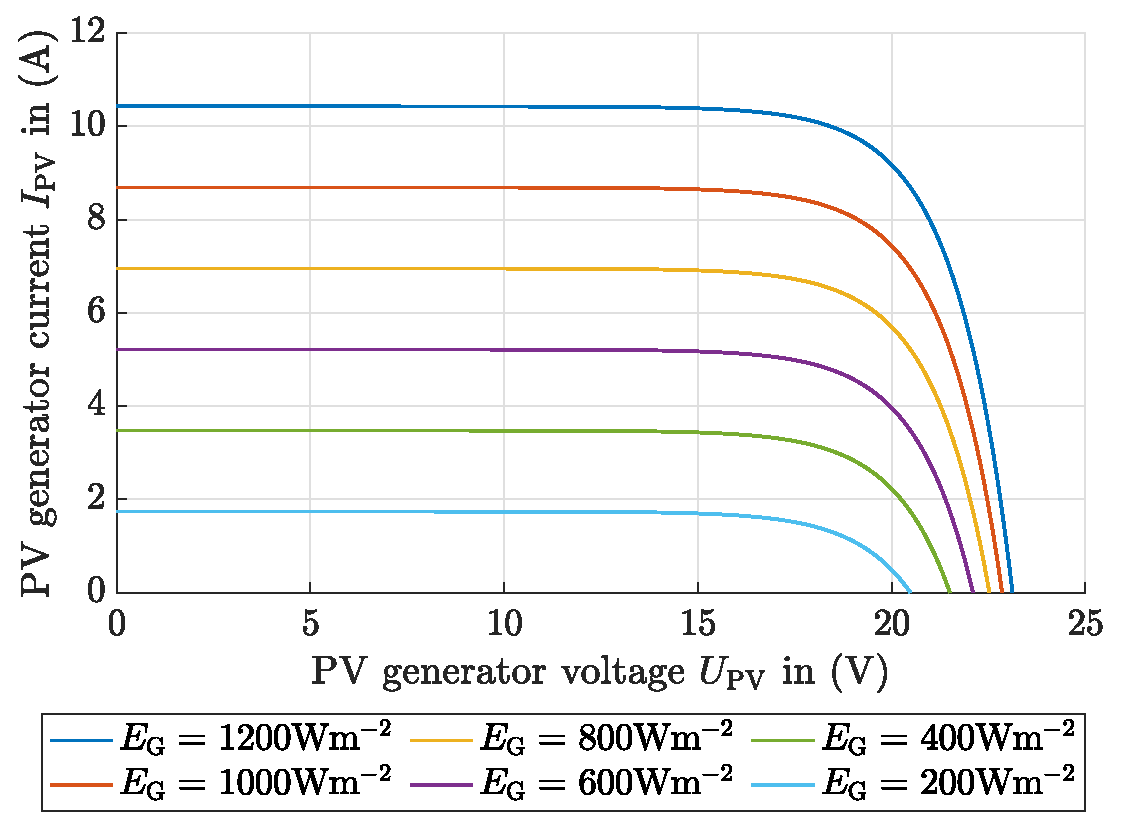
\includegraphics[width = 0.67\textwidth]{image_curr_volt_irr_das_energy.eps}
  	\caption{Modeled current-voltage characteristic of the DAS Energy DAS145PF PV generator, depending on the total irradiance onto its inclined surface $E_\mathrm{G}$. The PV cell temperature $\vartheta_\mathrm{C} = 25^\circ\mathrm{C}$ is assumed to be constant.}
	\label{fig:image_curr_volt_irr_das_energy}
\end{figure}

Now the associated power-voltage characteristics for different irradiance levels $E_\mathrm{G}$ of both PV generators can be calculated by using the equation (\ref{eq:p_pv_u}), as shown in the figures \ref{fig:image_power_volt_irr_ae_solar} and \ref{fig:image_power_volt_irr_das_energy}. As can be observed from a real PV generator, the power output $P_\mathrm{PV}$ decreases with lower irradiance levels $E_\mathrm{G}$. 
\begin{figure}[h!]
	\centering
  	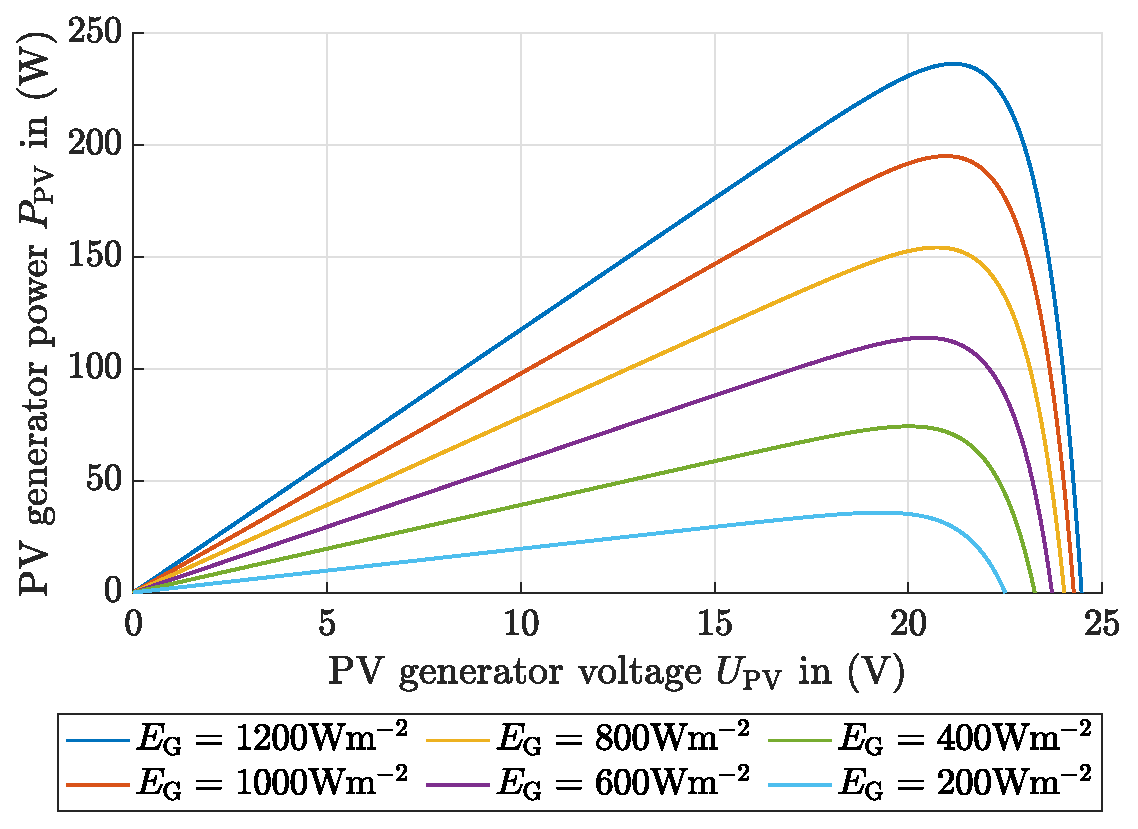
\includegraphics[width = 0.67\textwidth]{image_power_volt_irr_ae_solar.eps}
  	\caption{Modeled power-voltage characteristic of the AE Solar AE195SMM6-36 PV generator, depending on the total irradiance onto its inclined surface $E_\mathrm{G}$. The PV cell temperature $\vartheta_\mathrm{C} = 25^\circ\mathrm{C}$ is assumed to be constant.}
	\label{fig:image_power_volt_irr_ae_solar}
\end{figure}
\begin{figure}[h!]
	\centering
  	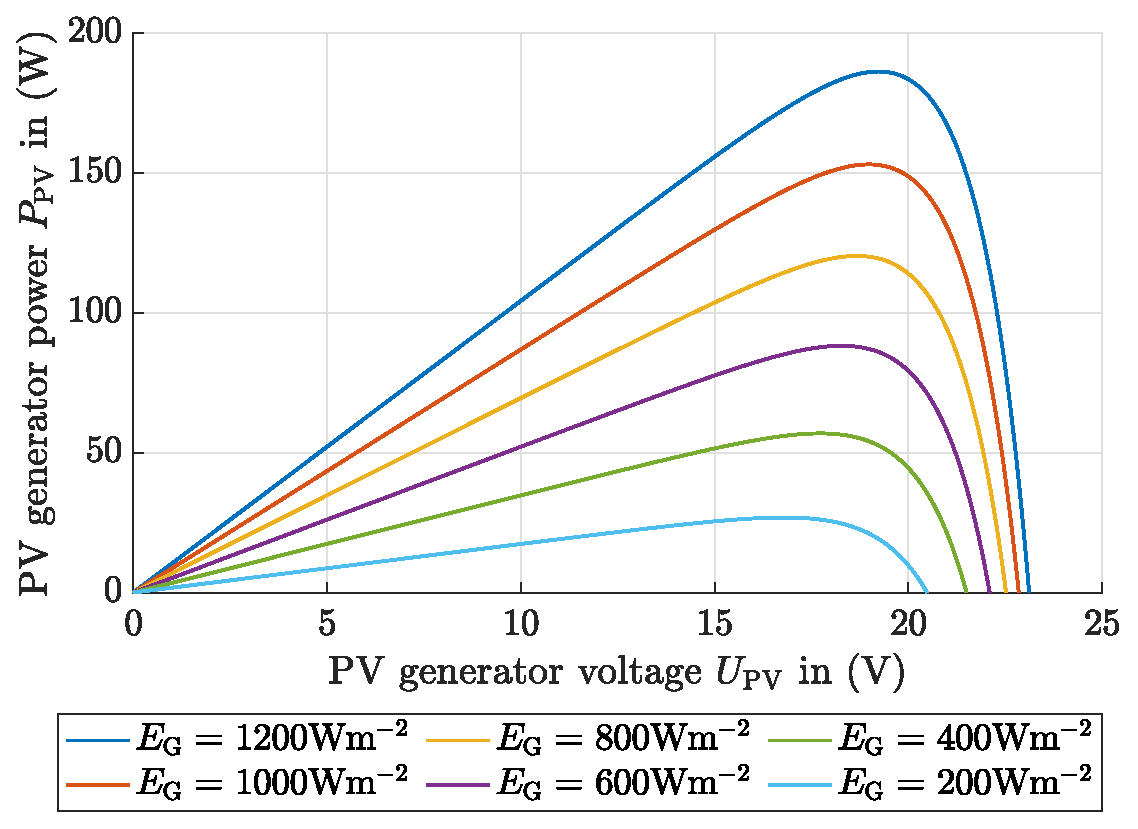
\includegraphics[width = 0.67\textwidth]{image_power_volt_irr_das_energy.eps}
  	\caption{Modeled power-voltage characteristic of the DAS Energy DAS145PF PV generator, depending on the total irradiance onto its inclined surface $E_\mathrm{G}$. The PV cell temperature $\vartheta_\mathrm{C} = 25^\circ\mathrm{C}$ is assumed to be constant.}
	\label{fig:image_power_volt_irr_das_energy}
\end{figure}

Another interesting behavior of the PV generators can be observed for different temperatures $\vartheta_\mathrm{C}$ of their PV cells. Due to the temperature increse of the semiconductors, the current $I_\mathrm{Ph} = I_\mathrm{SC}$ increses, however not as much as the voltage $U_\mathrm{OC}$ decreses. 
\begin{figure}[h!]
	\centering
  	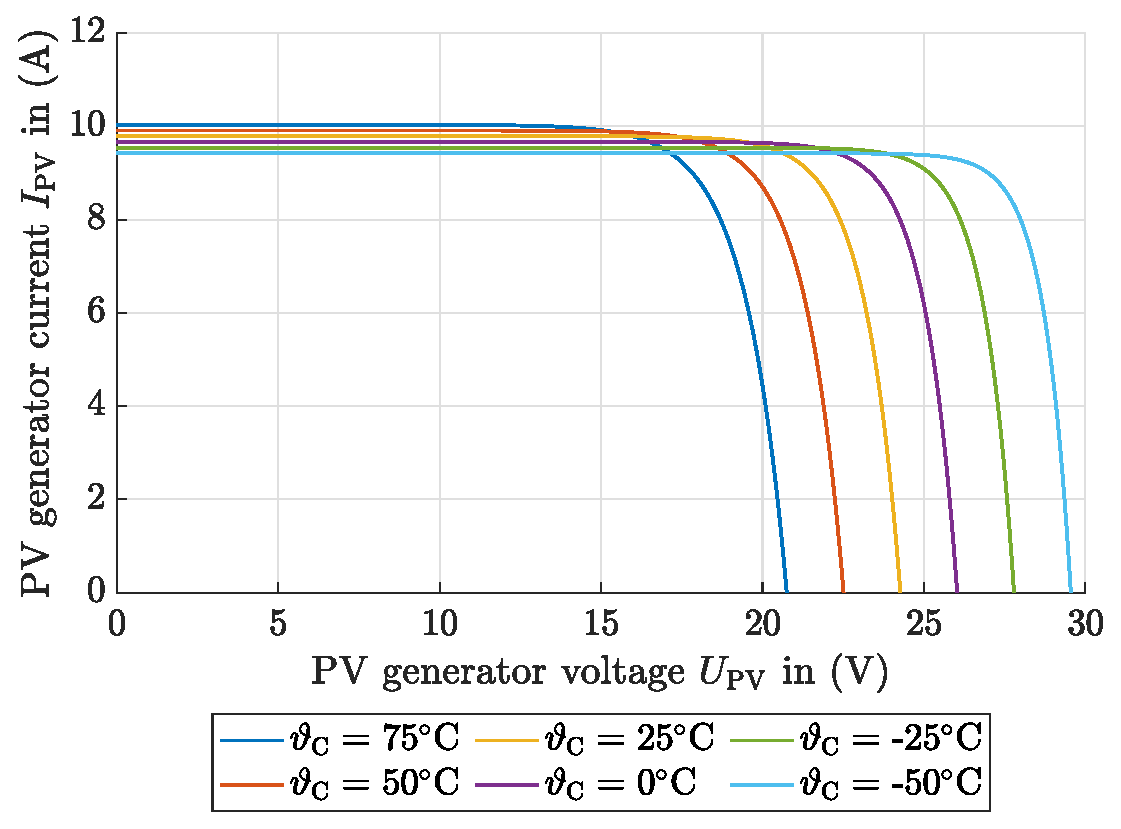
\includegraphics[width = 0.67\textwidth]{image_curr_volt_temp_ae_solar.eps}
  	\caption{Modeled current-voltage characteristic of the AE Solar AE195SMM6-36 PV generator, depending on its PV cell temperature $\vartheta_\mathrm{C}$. The total irradiance onto its inclined surface $E_\mathrm{G} = 1000\mathrm{Wm}^{-2}$ is assumed to be constant.}
	\label{fig:image_curr_volt_temp_ae_solar}
\end{figure}
\begin{figure}[h!]
	\centering
  	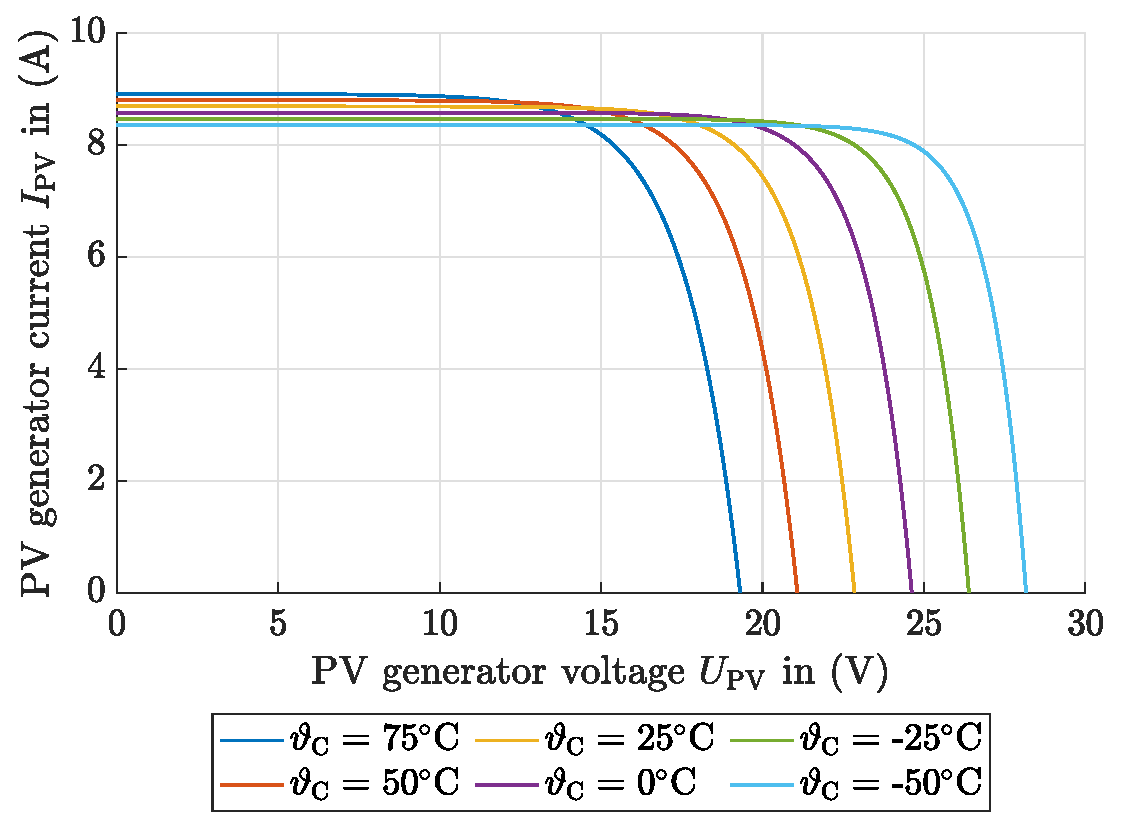
\includegraphics[width = 0.67\textwidth]{image_curr_volt_temp_das_energy.eps}
  	\caption{Modeled current-voltage characteristic of the DAS Energy DAS145PF PV generator, depending on its PV cell temperature $\vartheta_\mathrm{C}$. The total irradiance onto its inclined surface $E_\mathrm{G} = 1000\mathrm{Wm}^{-2}$ is assumed to be constant.}
	\label{fig:image_curr_volt_temp_das_energy}
\end{figure}
This finding results in an overall decrease in the power output $P_\mathrm{PV}$ of the PV generators for rising temperatures $\vartheta_\mathrm{C}$. Similarly, such behavior can be observed for decreasing temperatures $\vartheta_\mathrm{C}$. Here the overall power output $P_\mathrm{PV}$ increases. This is shown in the figures \ref{fig:image_curr_volt_temp_ae_solar} and \ref{fig:image_curr_volt_temp_das_energy}. When modeling a self-sufficient energy system, this factor must therefore not be neglected \cite{Mertens:2015}. 
\begin{figure}[h!]
	\centering
  	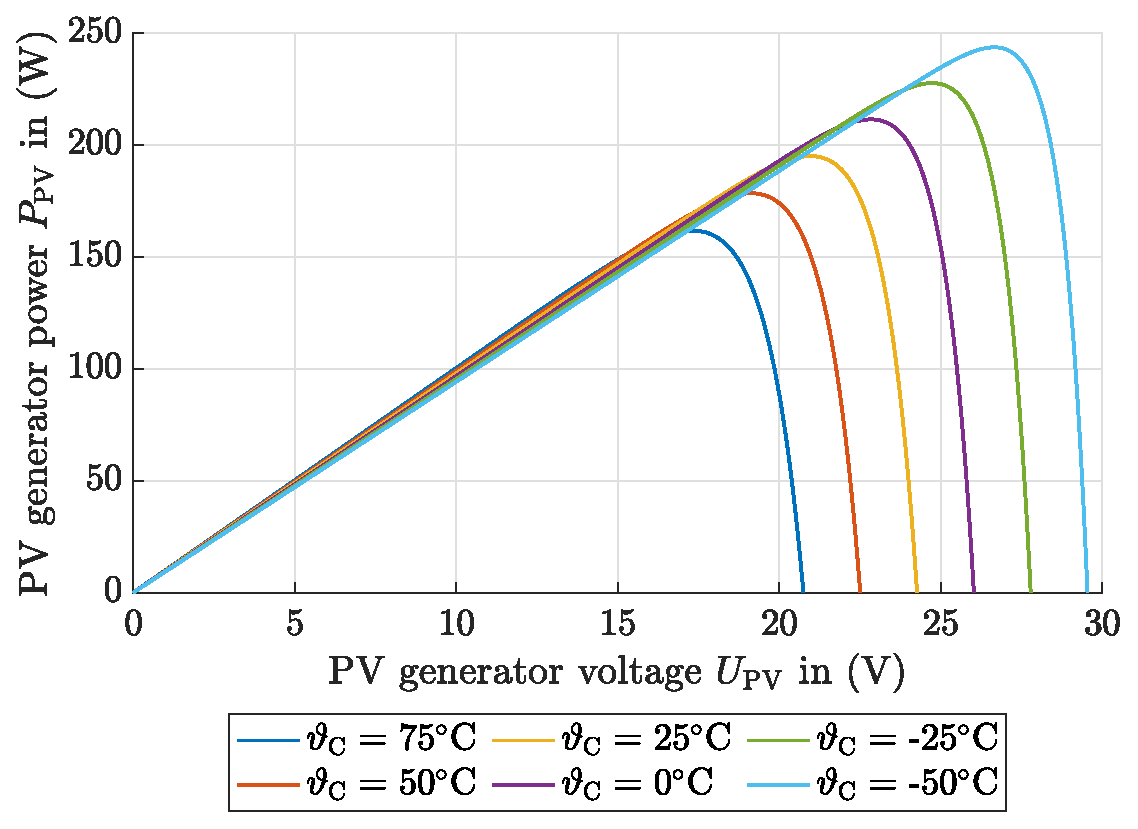
\includegraphics[width = 0.67\textwidth]{image_power_volt_temp_ae_solar.eps}
  	\caption{Modeled power-voltage characteristic of the AE Solar AE195SMM6-36 PV generator, depending on its PV cell temperature $\vartheta_\mathrm{C}$. The total irradiance onto its inclined surface $E_\mathrm{G} = 1000\mathrm{Wm}^{-2}$ is assumed to be constant.}
	\label{fig:image_power_volt_temp_ae_solar}
\end{figure}
\begin{figure}[h!]
	\centering
  	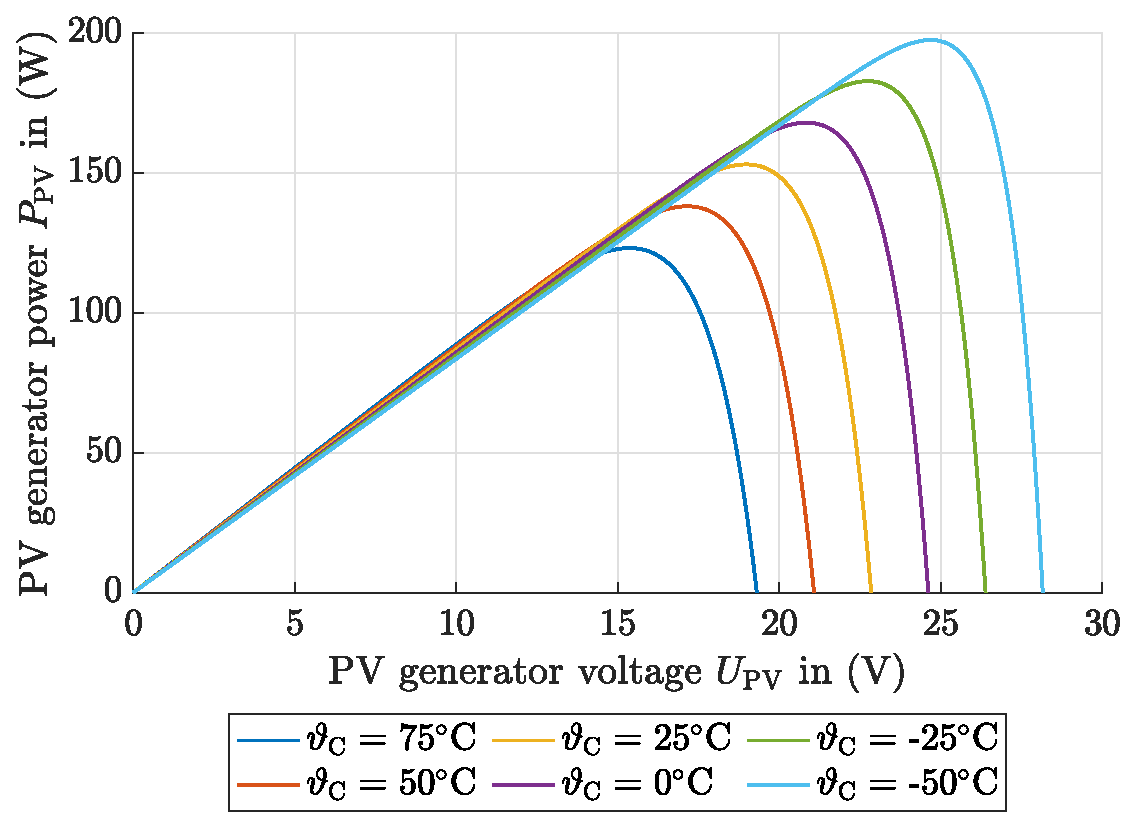
\includegraphics[width = 0.67\textwidth]{image_power_volt_temp_das_energy.eps}
  	\caption{Modeled power-voltage characteristic of the DAS Energy DAS145PF PV generator, depending on its PV cell temperature $\vartheta_\mathrm{C}$. The total irradiance onto its inclined surface $E_\mathrm{G} = 1000\mathrm{Wm}^{-2}$ is assumed to be constant.}
	\label{fig:image_power_volt_temp_das_energy}
\end{figure}

With the help of the aforementioned \MATLAB program, the ideality factors of the two PV generators were empirically determined in such a way that their power output at MPP for STCs corresponds to that in their data sheets. This resulted in an ideality factor of $m = 1,19045$ for the AE Solar AE195SMM6-36 PV generator and $m = 1,58972$ for the DAS Energy DAS145PF PV generator -- for an accuracy of two decimal places. 


 





